% Stand-in for IEEEtran so the paper can be measured before the class file
% arrives. Geometry chosen to approximate IEEEtran's text block; page counts
% from this build are indicative, not exact.
\documentclass[twocolumn,10pt]{article}
\usepackage[letterpaper,top=0.75in,bottom=1.0in,left=0.625in,right=0.625in,columnsep=0.25in]{geometry}
\usepackage{siunitx,booktabs,graphicx,amsmath,amssymb,threeparttable}
\usepackage[hidelinks]{hyperref}
\usepackage{url}
\newenvironment{IEEEkeywords}{\par\small\noindent\textbf{Index Terms}---}{\par}
\renewcommand{\markboth}[2]{}

\renewcommand{\abstractname}{Abstract}
\begin{document}
\twocolumn[\begin{@twocolumnfalse}
\title{Composite Timing Metrics Do Not Measure Warning Capability:
A Video-Blind Constant Matches the Eighth of Thirteen Teams, and the
Corrected Protocol Needs Correcting}

\author{Sudaroli~Dhananjeyan,
        Surya~G,
        and~Gomathi~D%
\thanks{S. Dhananjeyan is an Independent Researcher, Bengaluru, India
(e-mail: oli.sudar@gmail.com).}%
\thanks{S. G and G. D are with T. John Institute of Technology, Bengaluru,
India.}%
\thanks{Code, all submission files and the returned scores are available at
\url{https://github.com/sudaroli1/precrash}. The measurement data are archived
at \href{https://doi.org/10.17632/yjvr5c7v3n.1}{doi:10.17632/yjvr5c7v3n.1}.}}

\markboth{IEEE Transactions on Intelligent Transportation Systems}%
{Dhananjeyan \MakeLowercase{\textit{et al.}}: Composite Timing Metrics Do Not Measure Warning Capability}

\maketitle

\begin{abstract}
Traffic-accident anticipation is increasingly scored by composite metrics that
add an earliness term --- time-to-accident at a fixed risk threshold --- to
discrimination terms such as average precision and area under the ROC curve.
The composition fails structurally: the discrimination terms are bounded on the
unit interval, the earliness terms scale with clip length, and the earliness
terms are maximised by a constant risk score above the threshold --- a
submission that, deployed, would warn continuously. We measure the consequence
twice. On a live benchmark of 1{,}417 dashcam clips and thirteen teams, whose
labels are withheld and whose metric weights are undisclosed, a constant risk
score of $0.51$ that reads no pixels scores $2.35291$: it matches the
eighth-placed team at the precision the leaderboard displays and exceeds five of
thirteen entries including our own. Twenty-five such submissions, designed so
the undisclosed terms cancel under differencing, decompose the metric without
any label: discrimination contributes $0.35105$ and the two timing terms
$2.00186$, $5.70$ times as much. The same probes establish that four curves
crossing the threshold at the same frame score $0.091$ apart, a spread the
published definition cannot produce, so the stated formula does not reproduce
its own scorer. We then validate a corrected protocol on an independent corpus
of 1{,}500 annotated clips, half containing no collision. The pathology
reproduces --- a constant takes 99.9\% of the available earliness at exactly
chance discrimination --- and the cost it hides becomes measurable: such a
warning alarms for 60 minutes in every hour of ordinary driving. The protocol
behaves as predicted but is then beaten by a control that reads only the video
file's header, because clip-level conditioning cannot see a curve that is flat
within a clip. We replace it with a frame-level statistic, coverage of the
annotated actionable window against alarm duty cycle, under which the
video-blind family scores zero and a sighted model does not. Our own
ninth-placed entry, which scores below the constant, is the case study.
\end{abstract}

\begin{IEEEkeywords}
Accident anticipation, evaluation methodology, benchmark design, video-blind
baseline, time-to-accident, collision warning systems.
\end{IEEEkeywords}

\end{@twocolumnfalse}]
\section{Introduction}
\label{sec:intro}

Road traffic injury kills approximately 1.19 million people a year by the World
Health Organization's count~\cite{who2023}. Many of those deaths are
foreseeable in the seconds before they occur, which is why systems that
anticipate a collision --- rather than detect one after the fact --- are
pursued as a countermeasure, and why a growing literature reports how early
such systems can raise an alarm~\cite{zhang2025review}. Whether a reported
anticipation result establishes that a system could actually warn a driver is a
question about measurement, and it is the question this paper addresses.

Anticipation is increasingly scored by a composite metric: a weighted sum of
discrimination terms --- average precision (AP) and area under the ROC curve
(AUC) --- and an earliness term, the interval between alarm and collision read
at a fixed risk threshold. The composition is intuitive. An anticipator should
separate accident clips from ordinary driving and should raise the alarm early,
and summing terms that measure each seems a reasonable way to ask for both.

It is not, and the reason is a difficulty of type rather than of tuning. AP and
AUC are bounded on the unit interval; an earliness term counted in frames is
bounded only by the length of the clip. Summing a bounded quantity with an
unbounded one lets the unbounded one decide the ranking, and makes that ranking
depend on how the corpus was windowed. Worse, an earliness term read at a
threshold has a trivial global maximiser: a risk score that exceeds the
threshold at frame~0 and never falls attains, on every clip, the largest value
that clip admits. No method that reads the video can exceed it. A method can
only match it, and then compete on the bounded half.

That argument follows from the definitions alone. What has been missing is a
measurement of what it costs in practice, and the measurement is awkward to
obtain: the benchmarks using these metrics withhold their labels, and the
competitions using them do not publish the weights.

This paper supplies it twice over. On a live accident-anticipation benchmark
--- 1{,}417 dashcam clips, thirteen teams, a scorer we never saw --- a constant
risk score of $0.51$ that reads no pixels scores $2.35291$ against a winning
$2.50165$, matching the eighth-placed team at the precision the leaderboard
displays and exceeding five of thirteen entries. A family of submissions that
likewise read nothing, designed so that the undisclosed terms cancel when two
are differenced, then recovers the metric's parts from outside the competition:
the timing terms are worth \textbf{5.70 times} what discrimination contributes
to such a submission, and the score falls at almost exactly one sixtieth of a
point for every frame of delay.

Because that benchmark publishes no labels, it can show the metric being
exploited but cannot show anything being fixed. We therefore repeat the
measurement on an independent, fully annotated corpus of 1{,}500 clips, half of
which contain no collision. There the pathology reappears --- a constant takes
99.9\% of the available earliness at exactly chance discrimination --- and, for
the first time, the cost of the behaviour it rewards becomes measurable: a
warning that maximises this metric alarms for \textbf{60 minutes in every hour}
of ordinary driving.

The safety consequence is therefore not that the metric is untidy. The
submission maximising its earliness half is a warning that never turns off.
Whether a driver comes to trust a collision warning or to ignore it depends on
when it arrives relative to what the driver expects~\cite{abe2006alarm}, and a
warning that never stops carries no timing information at all. The metric
awards that behaviour its maximum and cannot do otherwise, because its timing
terms are defined only on clips where an accident occurs, so the burden such a
system imposes on ordinary driving falls entirely on the discrimination half.

We came to the question the awkward way: we built a training-free ensemble,
entered it in that competition, and placed ninth of thirteen. The paper is not
about that system --- it scores below the constant --- but it is what made the
metric worth examining, and it appears here as the case study.

\textbf{Contributions.} We report a measured demonstration on a live
benchmark: a video-blind constant matches the eighth-placed private score and
exceeds five of thirteen teams, our own included. We give a black-box
decomposition, in which video-blind probes built so that unknown terms cancel
under differencing separate a metric whose weights are undisclosed and whose
labels are withheld, recovering the discrimination floor, both timing terms,
the slope in the crossing frame and the accident-onset distribution. We show
that the published definition does not reproduce the scorer: four curves
crossing at the same frame, none dipping below it afterwards, score $0.091$
apart, where the stated formula requires equality. We then validate the
corrected protocol where ground truth exists; its predicted behaviour holds,
but it is beaten by a control reading only the video file's header, so we
replace its clip-level conditioning with a frame-level alarm statistic and show
that this orders submissions by what they can see. Every leaderboard score was
computed by the competition's scoring service against ground truth we do not
have; derived quantities are our arithmetic on those scores and are marked as
such.

One point of scope, because this paper prints a number beside other teams'
numbers. We make no claim about any other submission or published method: we
did not re-run anyone's system, and could not have evaluated it if we had,
because the labels are withheld from every entrant. Where a leaderboard score
is numerically identical to a control's, we state that arithmetic fact and draw
one inference --- the metric assigns the two submissions the same value. A
whole family of curves receives it, which is precisely the property under
examination.

\section{Background}
\label{sec:background}

\subsection{Where the metrics come from}

Vision-based accident anticipation was posed in its modern form by Chan
\textit{et al.}~\cite{chan2016dad}, who introduced the Dashcam Accident Dataset
together with the measure the field still reports: the interval between the
first frame at which a risk score crosses a threshold and the annotated onset
of the collision. Bao \textit{et al.}~\cite{bao2020ccd} contributed the Car
Crash Dataset and an uncertainty-based formulation, and Karim \textit{et
al.}~\cite{karim2022dsta} gave the reporting convention most subsequent work
adopts: average precision, mean time-to-accident over thresholds, and
time-to-accident at 80\% recall.

It is worth stating plainly what that convention gets right, because this paper
is about what happens when it is set aside. It reports a discrimination metric
alongside every timing metric, and it reads timing \emph{at a fixed operating
point} of the discrimination metric. A method therefore cannot buy
time-to-accident by alarming indiscriminately: the recall constraint holds it
to a fixed false-alarm behaviour before its timing is counted at all. The
repair proposed in Section~\ref{sec:protocol} is in large part a return to that
discipline.

Architectures built on this foundation run from supervised convolutional and
temporal models~\cite{chan2016dad, bao2020ccd, karim2022dsta} through
self-supervised formulations that reduce the dependence on scarce collision
labels~\cite{yao2019unsupervised, liu2026sctnet, zhong2025early}, to
training-free pipelines pairing a vision--language
model~\cite{radford2021clip} with a motion
signal~\cite{thakur2026modular, saha2026zeroshot, singh2026metadata} --- though
those target detection or classification and none reports a timing metric.

Two lines of work deserve particular attention, because they anticipate part of
this paper's subject. Pjetri \textit{et al.}~\cite{pjetri2025nondecreasing}
train with an objective requiring the predicted danger score to be
non-decreasing as the collision approaches, and Zou \textit{et
al.}~\cite{zou2026riskprop} introduce an adaptive monotonic constraint loss with
the same intent. Both are well-motivated responses to score oscillation and we
criticise neither. But both illustrate the hazard examined here: a risk score
constrained not to fall is, by construction, closer to the maximiser of a
threshold-crossing timing metric than a score free to fall. The metric cannot
separate the benefit of the constraint from the artefact of it, and neither
paper reports a control that would.

\subsection{From a convention to a single number}

Competitions need something the convention of~\cite{karim2022dsta} does not
supply: a total order over submissions. The natural way to obtain one is to sum
the metrics, and that is what the benchmark studied here
does~\cite{autopilot2026}, adding two threshold-crossing timing terms to
average precision and area under the ROC curve.

Summing is where the difficulty enters, and it is a difficulty of type rather
than of tuning. Average precision and area under the curve are bounded on the
unit interval; a time-to-accident measured in frames is bounded only by the
length of the clip. Adding them makes the sum depend on how the corpus was
windowed and lets the unbounded term decide the ranking.
Section~\ref{sec:why} develops the argument; Sections~\ref{sec:leaderboard}
and~\ref{sec:nexar} measure its magnitude.

\subsection{The missing control}

The check that exposes such a problem is a control that does not read the
input, and its value has been established repeatedly elsewhere: dataset
signatures strong enough to identify a photograph's
source~\cite{torralba2011bias}; models given only half the input scoring far
above chance on standard inference
corpora~\cite{gururangan2018artifacts, poliak2018hypothesis}, after which
partial-input baselines became standard practice; and tuned simple baselines
matching most recently published neural
recommenders~\cite{ferraridacrema2019progress}. In each case the control was
cheap, and in each case nobody had run it.

Accident anticipation has every precondition those episodes had. It reports a
timing metric whose maximiser is trivial, it is moving toward composite
single-number scores, and its newest benchmarks withhold labels --- so an
entrant cannot compute the discrimination half at all and must develop against
a locally computable proxy, the only candidate being the shape of one's own
risk curve, which a constant maximises.

The pathology has not gone unnoticed, but it has been noticed as an anomaly
rather than isolated. Zhao \textit{et al.}~\cite{zhao2025top} observe that the
standard calculation credits a false alarm in a safe scene with the interval to
some later, causally unrelated collision. Goldshmidt \textit{et
al.}~\cite{goldshmidt2025badas} report baselines making physically implausible
predictions nine to ten seconds ahead. Most directly, Caselli \textit{et
al.}~\cite{caselli2026flara} publish a table in which two established methods
record areas under the curve of $45.5$ and $41.0$ --- below chance --- beside
mean times-to-accident of $10.216$ and $10.263$ seconds. A method that cannot
separate accident clips from ordinary ones is there credited with ten seconds
of anticipation: this paper's argument, already legible in someone else's
results table. None of these accounts isolates the effect, and none reports
what a submission that reads nothing would score.

The nearest methodological precedent lies in an adjacent task. Korkut
\textit{et al.}~\cite{korkut2026blind} audit four traffic video
question-answering benchmarks by running vision--language models blind, and find
that removing the video consistently improves accuracy on one of them. That is
a control of exactly the kind advocated here, applied to multiple-choice
accuracy rather than to per-frame risk. We are not aware of an equivalent
control reported for the timing and discrimination metrics used in
anticipation, which is the gap this paper fills.

We state the scope of that observation precisely: it covers the works cited
here whose results tables we inspected directly. Four we consulted are behind
paywalls we could not open, and we exclude them rather than assume. It is not a
systematic audit of the field and we do not present it as one.

\subsection{What is and is not new here}

Monotonicity constraints on risk scores are prior
work~\cite{pjetri2025nondecreasing, zou2026riskprop} and this paper claims
none; so are training-free pipelines pairing a vision--language model with a
motion signal~\cite{thakur2026modular}. Nor is the general idea that a
benchmark can be satisfied by a degenerate submission new, and the suspicion
that time-to-accident is inflatable has been voiced
before~\cite{zhao2025top, goldshmidt2025badas, caselli2026flara}, as has a blind
control on an adjacent traffic-video task~\cite{korkut2026blind}. What is new is
the measurement of how far it goes on this class of metric, a probe methodology
that decomposes such a score from outside the competition holding the labels,
and an evaluation protocol that has been tested against adversarial controls,
found insufficient, and repaired.

\section{The Benchmark, the Controls and the Probes}
\label{sec:method}

This section describes the benchmark whose metric is under examination and the
two families of submission with which we measured it. Neither family reads a
video frame.

\subsection{The competition}
\label{sec:competition}

Measurements were made on Zero-shot Accident Anticipation, a public competition
hosted on Kaggle~\cite{autopilot2026}. It ran from 17 February to 15 April
2026, drawing 59 entrants of whom 20 submitted, forming 13 teams across 194
submissions. Late submission remains open and is scored against the same
splits, which is how the experiments of Section~\ref{sec:leaderboard} were run
after the closing date. Every figure quoted here was read from the
competition's own pages on 31 August 2026.

Two properties make it a suitable instrument. The organisers hold the labels
and compute every score, so nothing reported here depends on our own
implementation of a metric. And a submission is a plain list of numbers per
clip, so it need not contain a model at all --- which is what makes a
video-blind control submittable.

The corpus is a curated 1{,}417-clip subset of MM-AU~\cite{fang2024mmau}, every
clip exactly 150 frames at 30\,fps. The published test file carries an
identifier, a video identifier, a start and end frame, and a caption. There is
no label, no accident time and no alert time.

One consequence deserves emphasis, because the rest of this paper turns on it.
Average precision, area under the ROC curve, a false-positive rate, and any
time-to-accident measured to a true onset are \emph{not computable by any
entrant}. An entrant wanting to measure progress locally must substitute
something, and the only quantities computable from a submission alone are
properties of the risk curve's own shape --- the frame at which it crosses the
threshold, whether it falls back, how steeply it rises. We did exactly this,
and Section~\ref{sec:leaderboard} measures what that proxy was worth. A second
consequence we identify without quantifying: the 79 distinct captions describe
outcomes (``lead vehicle stops'', 146 clips; ``a vehicle controls loss'', 144),
and they are supplied at inference time, so a method conditioned on them has
access to the outcome it is asked to anticipate.

\subsection{The metric, as published}
\label{sec:metric}

The evaluation page defines the score as a weighted sum of four quantities,
\begin{equation}
\text{score} = w_{\text{AP}}\text{AP} + w_{\text{AUC}}\text{AUC}
 + w_{\text{TTA}}\text{TTA@0.5} + w_{\text{STTA}}\text{STTA@0.5}
\end{equation}
with the weights fixed by the organisers and not disclosed. Positives are
accident clips, negatives ordinary driving. The timing terms are read at a risk
threshold of $0.5$:
\begin{align}
\text{TTA@0.5} &= \max\{\, t_{ai} - t_a \mid p_{t_a} > 0.5,\ 0 \le t_a \le t_{ai} \,\} \\
\text{STTA@0.5} &= \max\{\, t_{ai} - t'_a \mid p_t > 0.5\ \forall\, t \in [t'_a, t_{ai}] \,\}
\end{align}
where $t_{ai}$ is the accident start frame and $t_a$ the first frame at which
the risk score exceeds the threshold. STTA additionally requires the score to
remain above the threshold continuously from $t'_a$ to $t_{ai}$.

Three observations follow from these definitions alone, before any measurement.

\emph{First}, AP and AUC are bounded on the unit interval, while TTA and STTA
are counted in frames and bounded only by $t_{ai}$ --- hence by how the corpus
was windowed. The four terms are not commensurable, and their sum inherits the
scale of the larger pair.

\emph{Second}, both timing terms are maximised by the same trivial submission.
A risk score exceeding $0.5$ at frame~0 and never falling has $t_a = 0$ and
satisfies the continuity condition on every clip, attaining
$\text{TTA} = \text{STTA} = t_{ai}$, the largest value each clip admits. No
submission can exceed it; one can only match it, and then compete on AP and
AUC.

\emph{Third}, neither timing term reads the magnitude of the score, only
whether it stands above $0.5$. A submission that is barely committed and one
that is certain receive identical timing credit, so the metric offers no
incentive to calibrate.

\subsection{Video-blind controls}
\label{sec:controls}

A video-blind submission is one whose risk curve is a function of the frame
index alone: identical for every clip, computed without opening a frame. We use
a family rather than a single curve, because one flattering curve invites the
objection that the comparison was chosen to flatter it. The family comprises
constants at $0.51$ and $0.99$; a curve held at $0.49$, which never crosses; a
linear ramp; logistic curves centred at frames 60, 75, 90 and 105; step
functions rising from $0.49$ to $0.51$ at frames 0, 10, 25, 50, 75, 100, 125
and 140, plus a calibration step at frame 76; a curve that crosses at frame~0
then drops back, and one that crosses and dips across frames 50--59; and two
graded curves. That is 21 distinct shapes submitted as 25 files --- four were
sent twice, and the repeats agree to within $3\times10^{-5}$, which is a check
on the scoring service and not only on our bookkeeping.

Before spending a submission slot we regenerated the organisers' sample file
from its own parsed values and compared it byte for byte against the
distributed file: identical. A scoring anomaly therefore cannot be attributed
to our file writer.

\subsection{Probes that isolate the terms}
\label{sec:probes}

The decomposition rests on one observation. Every video-blind submission is
identical across clips, so --- provided the scorer reduces each curve to one
clip-level score by any deterministic function of that curve --- every member
of the family produces an all-way tie among clips, and therefore earns
identical AP and identical AUC. Whatever those terms are worth, they are worth
the same to all of them, and \emph{they cancel exactly in any difference
between two members}.

That turns the leaderboard into an instrument. Three probes suffice. A curve
held at $0.49$ never crosses, so both timing terms are zero and its score is
the discrimination floor alone. A curve at $0.51$ in frame~0 and $0.49$
thereafter crosses once and then falls, earning the time-to-accident term but
forfeiting the stable one. A constant $0.51$ earns both. Differencing the three
gives each term separately. A fourth probe, holding $0.51$ throughout except
for a dip across frames 50--59, moves the stable term's reference point while
leaving the first crossing untouched, and serves as a consistency check.

The step family measures the score's dependence on the crossing frame directly,
giving a second and independent route to the same quantity. Two routes to one
number is what makes the result safe to report.

\begin{table}[t]
\caption{The final private leaderboard as published, with this work's
video-blind controls below the rule. The controls were submitted after the
closing date and scored by the same service against the same private split;
they are not leaderboard entries and are not ranked.}
\label{tab:lb}
\centering
\begin{tabular}{@{}rlc@{}}
\toprule
rank & entry & private score \\
\midrule
1 & CVLAB & 2.50165 \\
2 & BUPT MIC Lab & 2.46234 \\
3 & Tianhao Zhao & 2.42361 \\
4 & cr-tfx & 2.41555 \\
5 & wtiaw\_tiaw & 2.39725 \\
6 & IsaacfI & 2.39027 \\
7 & yyttll & 2.36844 \\
8 & Paulini38 & \textbf{2.35291} \\
9 & \emph{our entry} & 2.00585 \\
10 & Song\_Ren & 1.46008 \\
11 & WDL & 1.35992 \\
12 & YooHyun.2 & 1.04203 \\
13 & Ratnachand Kancharla & 1.03913 \\
--- & benchmark row on the leaderboard & 0.58333 \\
\midrule
\multicolumn{3}{@{}l}{\emph{video-blind controls (this work)}} \\
--- & constant $0.51$ at every frame & \textbf{2.35291} \\
--- & constant $0.99$ at every frame & 2.35291 \\
--- & linear ramp $0.000 \to 1.000$ & 1.06725 \\
--- & organisers' sample, resubmitted & 1.04203 \\
--- & never crosses ($0.49$ throughout) & 0.35105 \\
\bottomrule
\end{tabular}
\end{table}

\begin{table}[t]
\caption{Probes designed so the discrimination terms cancel under differencing,
and the components recovered from them. The ratio compares the timing terms at
their maximum against discrimination at chance.}
\label{tab:decomp}
\centering
\begin{tabular}{@{}lc@{}}
\toprule
probe & private score \\
\midrule
never crosses ($0.49$ throughout) & 0.35105 \\
crosses at frame 0, then drops & 1.22698 \\
crosses at frame 0, dips 50--59 & 1.85347 \\
constant $0.51$ & 2.35291 \\
\midrule
component & contribution \\
\midrule
AP $+$ AUC, to a video-blind submission & 0.35105 \quad ($1.00\times$) \\
TTA@0.5, saturated & 0.87593 \quad ($2.50\times$) \\
STTA@0.5, saturated & 1.12593 \quad ($3.21\times$) \\
\textbf{timing terms together} & \textbf{2.00186} \quad ($\mathbf{5.70\times}$) \\
\bottomrule
\end{tabular}
\end{table}

\begin{table}[t]
\caption{Four curves that all first exceed $0.5$ at frame 75 and never fall
below it afterwards; the three step-like ones hold identical values at frames
74 and 75. Under the published definition they must score identically. They
span $0.09093$.}
\label{tab:anomaly}
\centering
\begin{tabular}{@{}lcc@{}}
\toprule
curve & private score & vs.\ step \\
\midrule
graded run-up ($0 \to 0.49$, then $0.51$) & 1.12964 & $+0.02519$ \\
step ($0.49 / 0.51$) & 1.10445 & reference \\
graded throughout ($0.000 \to 1.000$) & 1.06725 & $-0.03720$ \\
graded run-out ($0.49$, then $0.51 \to 0.99$) & 1.03871 & $-0.06574$ \\
\midrule
step at frame 76 (one-frame calibration) & 1.08779 & $-0.01666$ \\
\bottomrule
\end{tabular}
\end{table}

\section{Results on the Live Benchmark}
\label{sec:leaderboard}

Every score in this section was computed by the competition's scoring service
against ground truth we do not hold. We implemented none of the four metrics.
Quantities derived from those scores --- the decomposition, the fit, the ratios
--- are our own arithmetic and are identified as such.

\subsection{A video-blind constant on the official leaderboard}

Table~\ref{tab:lb} reproduces the final private leaderboard as published, with
the video-blind controls below the rule: submitted after the closing date and
scored by the same service against the same private split. They are not
leaderboard entries.

A constant risk score of $0.51$ scores \textbf{2.35291}. That equals the
eighth-placed team's score at the five decimals the leaderboard displays,
exceeds five of the thirteen teams including our own, and falls $0.14874$ short
of the winner. Per the scope stated in Section~\ref{sec:intro}, the only
inference we draw from the coincidence at eighth place is that the metric
assigns those two submissions the same value; a whole family of curves --- every
curve above $0.5$ at frame~0 that never dips --- receives it, and we infer
nothing about what any team submitted.

We quote the difference before the ratio deliberately. The metric is a weighted
sum with no meaningful origin, so a ratio of two scores can be made to say
almost anything by shifting the scale. The difference of $0.14874$ and the
decomposition below are scale-free; that the constant reaches 94.1\% of the
winning score is a convenience, not evidence.

One further row is worth stating plainly. The organisers' own sample
submission, resubmitted byte for byte, scores $1.04203$, while the benchmark row
displayed on the leaderboard scores $0.58333$ --- so those are not the same
file, and the sample submission is not the origin of the published benchmark
score.

\subsection{Decomposing the score}

Because every video-blind submission is identical across clips, all of them
induce the same ordering over clips and earn the same AP and the same AUC,
which therefore cancel in any difference between two of them
(Section~\ref{sec:probes}). Differencing the probes separates the terms;
Table~\ref{tab:decomp} gives both the probe scores and the components recovered
from them.

Read the ratio precisely. It compares the timing terms at their maximum against
the discrimination terms at chance, not maximum against maximum. The maxima
ratio is not identifiable from outside, because the weights are undisclosed,
but it is bounded: the winner's discrimination terms are worth at least
$0.14874 + 0.35105 = 0.49979$, giving a maxima ratio of at most $4.01$. Both
framings say the same thing, and the measured statement is the safer one --- a
submission that reads nothing collects $2.00186$, and the best discrimination
anyone demonstrated on this benchmark added $0.14874$ to it.

Two further readings follow. A constant at $0.51$ and a constant at $0.99$
score identically, so the metric reads only whether the curve stands above the
threshold and never by how much. And the dip probe scores $1.85347$ where the
per-frame stable-timing coefficient predicts $1.79041$, so the additive split of
the timing total into its two parts is close but not exact; we report the split
with that tolerance attached. The total itself is measured directly between two
flat curves and does not depend on the split.

\subsection{The score is linear in the crossing frame}

Over the region in which the alarm still precedes the accident in every clip,
the score falls by $0.016647$ for each frame of delay --- one point per $60.1$
frames, or $0.4994$ per second at 30\,fps (Fig.~\ref{fig:linear}). A dedicated
one-frame experiment confirms the slope directly: a step at frame 75 scores
$1.10445$ and a step at frame 76 scores $1.08779$, a difference of $0.01666$
against $1/60 = 0.016667$.

The line was then asked to predict curves it had not seen. Three logistic
curves crossing at frames 60, 75 and 90 are predicted to within
$6.4\times10^{-3}$, the closest to $6\times10^{-5}$. A fourth, crossing at frame
105, lies beyond the fitted region where the curve has already begun to bend;
the model is not expected to hold there and we report it rather than omit a
held-out point that missed.

\subsection{The published definition does not reproduce the scorer}
\label{sec:anomaly}

One result does not fit, and we report it rather than smooth it. A linear ramp
crosses the threshold at frame 75, exactly as a step function does, and scores
$0.037$ lower. That gap is $2.24$ frames of slope, not an integer, so it cannot
be a crossing-frame effect. We therefore submitted a diagnostic family holding
the crossing frame at 75 and varying only the shape away from it
(Table~\ref{tab:anomaly}).

The four curves at the head of that table cross at the same frame and never
fall back, and the three step-like ones hold identical values at frames 74 and
75. Under the metric as published they must score identically: both timing
terms are functions of threshold crossings alone, and video-blind curves are
identical across clips, so the discrimination terms cannot separate them
either. They span $0.09093$, which is $5.5$ frames of slope.

We do not have an explanation and state the two candidates rather than choose.
Either the discrimination terms are not invariant to curve shape among
video-blind submissions --- which would weaken the cancellation argument of
Section~\ref{sec:probes}, though it is hard to reconcile with a step at frame
140 and a flat $0.49$ scoring identically despite very different frame
orderings --- or the timing terms read something beyond the first crossing that
the three agreeing curves share and the ramp does not.

Either way one conclusion is available without resolving it, and it is a
finding in its own right: \textbf{the benchmark's published formula does not
reproduce its scorer}. An entrant cannot compute this competition's score from
its stated definition even given the labels. The headline result is unaffected,
because the constant and the floor are both flat curves whose difference is
measured directly; what carries a caveat is the split of the timing total.

\subsection{A property of the withheld ground truth, recovered}

For a step at frame $k$, both timing terms equal $\max(t_{ai} - k, 0)$ on each
contributing clip, so the score above the floor is $c\,\mathbb{E}[\max(t_{ai} -
k, 0)]$ with $c$ the sum of the two timing weights. Differentiating, the slope
at $k$ is $-c\,P(t_{ai} > k)$: the slope measures the survival function of the
accident-onset distribution, scaled. The leaderboard is therefore reporting, one
submission at a time, the shape of an annotation no entrant has seen.

The initial segment estimates $c$ at $0.016667$, and dividing the timing total
by $c$ gives a mean onset of $120.1$ frames --- about four seconds into a
five-second clip. This explains mechanically why the constant does so well
here: because the accident is always late in the window, an alarm at frame~0 is
credited with roughly 120 frames of anticipation on every clip.

Two caveats belong with it. Under the model the magnitude of the slope must be
non-increasing in $k$, because a survival function cannot rise; it is not, by
roughly ninety times what five-decimal rounding permits, and we suspect the
same second-order effect as in Section~\ref{sec:anomaly}. And when $k$ exceeds
$t_{ai}$ the maximum in the published definition is taken over an empty set and
is undefined; we assume the scorer takes it as zero. We deliberately do not
separate the weights from the metric values: every quantity above is a product
of the two, and the positive rate cancels identically out of the onset ratio,
so this measurement says nothing about what fraction of the corpus contains an
accident.

\subsection{The case study: our own entry}
\label{sec:casestudy}

We reached this question by entering the competition, with a training-free
ensemble combining CLIP-based semantic scoring, optical-flow motion energy and
a third channel, fused by grid-searched weights with monotone clamping and
temporal post-processing. It placed ninth of thirteen at $2.00585$ ---
\emph{below the video-blind constant}. Auditing it against its released code
rather than against our description of it found three defects of exactly the
kind this paper is about. The third ``semantic'' channel is not a captioning
model: it thresholds the same frame-difference statistic the motion channel
uses and selects one of three fixed strings, so the ensemble has two
independent inputs rather than three --- which is why that channel posts an
\emph{earlier} mean crossover than the full ensemble. The monotone clamp forces
precisely the condition STTA tests, so any report of STTA compliance measures
that the clamp executed. And a temporal resampling stage evaluated the curve at
index $\alpha t$ while emitting it at $t$, so the score reported for frame $t$
was computed from a frame that had not yet arrived; a six-frame gain once
attributed to it is withdrawn, and the released configuration disables the
stage. No measurement above depends on this system. It is here because a
critique of evaluation practice written by authors who had not audited their
own entry would be worth less.

\begin{figure}[t]\centering
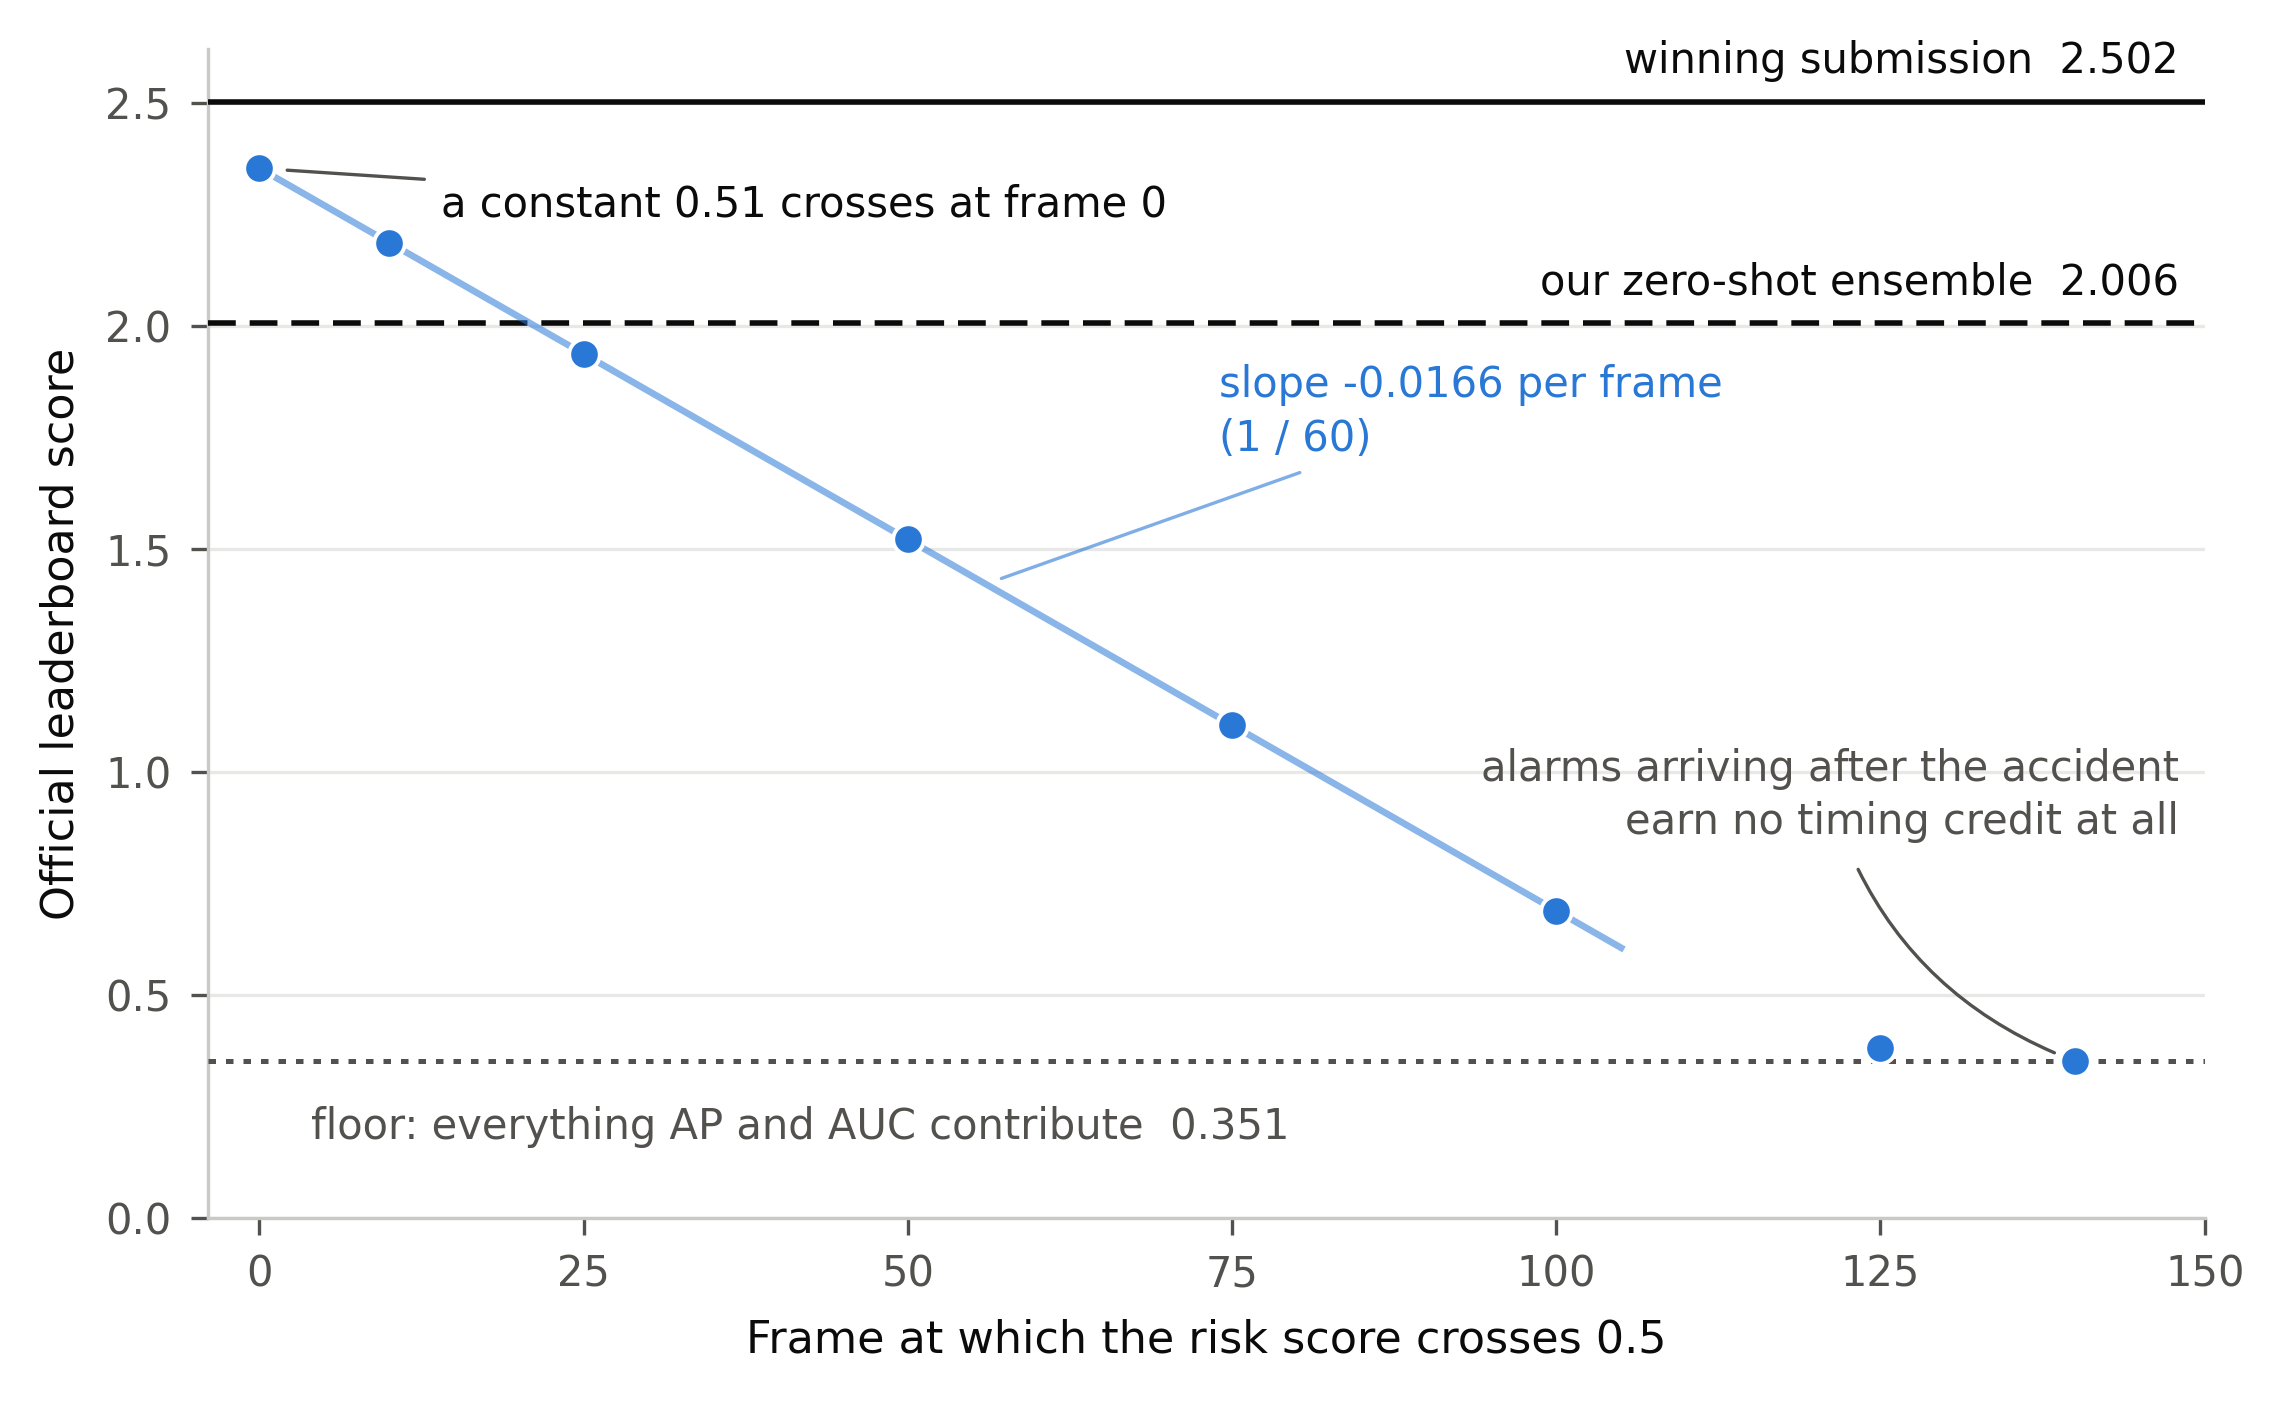
\includegraphics[width=\columnwidth]{media/image2.png}
\caption{The official score is a straight line in the frame at which the alarm
fires. Points are video-blind submissions scored by the organisers; the fit is
over crossings up to frame 100. A constant crosses at frame 0.}
\label{fig:linear}\end{figure}
\section{Validation on a labelled corpus}
\label{sec:nexar}

The competition publishes no labels. That is what makes its metric exploitable
from outside, and it is also what makes the corrected protocol of
Section~\ref{sec:protocol} untestable there: every repair in it is stated in
terms of quantities --- a false-positive rate, an annotated collision time, a
fixed operating point --- that the benchmark does not expose. A protocol that
cannot be run is a proposal, not a result.

This section runs it, on a corpus that is independent of the competition and
fully annotated: the Nexar collision-prediction training split of 1,500 dashcam
clips, 750 of which contain a collision and 750 of which are ordinary driving.
Every positive clip carries two annotations, a collision time $t_{\text{ev}}$
and an alert time $t_{\text{al}}$ marking the earliest moment at which a driver
could still have acted. Three things follow that the competition does not
allow. Average precision and area under the curve become measured quantities
rather than a floor recovered by differencing. Earliness is measured to the
annotated collision rather than to the end of the window. And because half the
corpus contains no collision at all, the cost a warning imposes on ordinary
driving becomes a number rather than an argument.

\subsection{Setup}

The video-blind family of Section~\ref{sec:controls} is regenerated for clips
that differ in length and frame rate: each curve is a closed-form expression in
the frame index, and a generator is given only the clip's frame count and frame
rate, so a curve that wanted a label could not read one. The published metric
is implemented exactly as Section~\ref{sec:metric} states it, with
$t_{ai}$ resolved to the annotated collision in each clip's own timebase.

Against these we place a sighted baseline. It is deliberately modest and no
claim here depends on its accuracy; its only job is to read pixels, so that the
protocol has something sighted to separate from the blind. Five motion
statistics are computed per frame at a fixed \SI{7.5}{\hertz} --- bulk and
localised frame difference, frame difference restricted to the lower-centre of
the image, luminance and its change --- and a logistic model over causal
summaries of them predicts whether the current moment lies inside the annotated
actionable window $[t_{\text{al}}, t_{\text{ev}}]$. The split is 600 clips for
training and 300 held out, fixed before any modelling. Every feature at time
$t$ is a function of samples at or before $t$; the property is asserted by
perturbation rather than assumed, by requiring that altering the tail of a clip
leave every earlier feature bit-identical.

Two properties of the corpus are worth stating before any score, because both
bear on the argument. Its clips carry \textbf{36 distinct frame rates} between
\SI{23.6}{fps} and \SI{31.0}{fps}, so an earliness term counted in frames is
summing quantities of different duration within a single dataset. And its
collisions occur between \SI{3.03}{\second} and \SI{56.80}{\second} into their
clips, an \textbf{18.7-fold spread} in the largest earliness any submission can
collect. The scale objection of Section~\ref{sec:why}(a) does not require two
differently windowed corpora to demonstrate; one is enough.

\subsection{The metric behaves the same way, and the corpus leaks}

Table~\ref{tab:nexar-blind} scores the video-blind family on all 1,500 clips. A
constant risk score of $0.51$ collects \SI{19.09}{\second} of TTA@0.5 and
\SI{19.09}{\second} of STTA@0.5 --- \textbf{99.9\% of the \SI{19.10}{\second}
ceiling} the corpus admits --- while scoring exactly $0.500$ on both
discrimination terms, which is what a constant must score. The result of
Section~\ref{sec:leaderboard} is therefore not a property of one organiser's
scorer. It follows from the composition, and it reappears wherever the
composition is used.

One finding here was not anticipated by the analysis of
Section~\ref{sec:why} and could not have been made on the competition corpus.
Clip duration alone separates collisions from ordinary driving at an AUC of
$0.537$; frame count alone at $0.548$; and \textbf{the frame rate of the video
file alone at $0.533$}. A submission that opens the container header, reads how
fast the file was encoded, and never decodes a frame scores above chance.

This is a property of how the corpus was assembled rather than of the metric,
but it has a direct consequence for anyone evaluating on it: a discrimination
score slightly above chance is not evidence that a method has seen anything.
We therefore add a \emph{metadata-only} control --- a model given the file's
frame rate and duration and nothing else --- to the protocol of
Section~\ref{sec:protocol}, alongside the video-blind one. We did not know to
ask for it before running this study, which is itself the argument for running
controls rather than reasoning about them.

\subsection{What each submission earns on held-out clips}

Table~\ref{tab:nexar-held} scores everything on the same 300 held-out clips.
Under the published metric the ordering is inverted with respect to what the
metric is supposed to reward. The sighted model is the only submission that
discriminates at all, at AUC $0.671$ against $0.500$ for every blind curve, and
it earns \SI{0.045}{\second} of TTA. The constant, at chance discrimination,
earns \SI{18.86}{\second}. \textbf{The composition pays blindness 424 times
better than sight.}

The mechanism is the one Section~\ref{sec:why}(c) identifies: neither timing
term reads the magnitude of a score, only whether it stands above $0.5$. A
model trained to be calibrated on a corpus where roughly one frame in fifty is
inside an actionable window produces probabilities that rarely cross a
threshold set at one half, and is penalised for it. A submission that is simply
pinned above the threshold is not.

\subsection{The protocol, tested and found insufficient}

Section~\ref{sec:protocol} makes a specific and falsifiable prediction about
its own two halves: bounding the earliness term normalises it into the unit
interval but \emph{does not} remove the constant as maximiser, and only
conditioning on a fixed operating point of the discrimination metric does.

That prediction holds exactly. Under bounding alone the constant scores
$1.0000$ --- it still takes the whole of the available anticipation, now
expressed as a ratio. Conditioned at a false-positive rate of 10\% it scores
$0.0000$, because there is no threshold at which it detects anything without
detecting everything. Had the constant failed at the bounding step instead,
either the implementation or the analysis of Section~\ref{sec:why} would have
been wrong.

The protocol does not survive the metadata-only control, and it fails under
both readings of its own averaging rule. Read as written --- normalised
earliness averaged over the positives a submission detects --- the
metadata-only control scores a \textbf{perfect $1.0000$} against the sighted
model's $0.0611$, while detecting 14 of 150 positives to the sighted model's
35. Averaged instead over all positives, charging an undetected one zero, it
scores $0.0933$ against $0.0143$. Either way the submission that reads the file
header outscores the one that reads the road, under the protocol proposed to
prevent exactly this.

The reason is structural and we had not seen it. Conditioning uses a
\emph{clip-level} discrimination metric, which asks whether a submission ranks
collision clips above ordinary ones. It cannot ask whether the alarm, within a
clip, is raised at a useful moment. A curve that is flat across a clip passes
clip-level conditioning on whatever discrimination it has, and then collects
maximal earliness on every clip it detects at all, because a flat curve above
threshold has been above threshold since the first frame.

The two readings above are the second defect. Averaging over detected
positives only --- the natural reading of Section~\ref{sec:protocol}, item 2
--- lets a submission buy a perfect score by detecting almost nothing, which is
precisely what the metadata-only control did. Earliness that is never
delivered, because the alarm was never raised, is not earliness; the statistic
must be averaged over all positives. That repair is necessary and, as the
figures above show, nowhere near sufficient.

\subsection{The repair: measure the alarm, not the ranking}

Both defects have the same root. The protocol conditions on a quantity computed
per clip, while the thing a warning system does --- and the burden it imposes
--- happens per frame. The repair is to measure the alarm itself. Partition
every frame of the corpus into two populations:

\begin{itemize}
\item \textbf{actionable}: frames of a collision clip inside
  $[t_{\text{al}}, t_{\text{ev}}]$, the interval the annotators mark as still
  avoidable;
\item \textbf{non-actionable}: every frame of every ordinary-driving clip, plus
  frames of a collision clip before $t_{\text{al}}$.
\end{itemize}

Frames after the collision belong to neither: nothing is being anticipated
there, and charging them would reward a curve for switching off after an event
it cannot know has occurred. Then report two rates at a common threshold ---
\emph{coverage}, the share of actionable time during which the alarm is raised,
and \emph{duty cycle}, the share of non-actionable time during which it is
raised --- and summarise by coverage at a capped duty cycle.

Fig.~\ref{fig:woc} sweeps both over every threshold. The diagonal is the
no-skill line, and the permanent alarm sits on it, at the top right corner: it
covers every actionable moment and alarms through every other one. That corner
is the point the published composite scores at its maximum.

Table~\ref{tab:nexar-held} gives the summary. At a duty cycle capped at 10\%
the entire video-blind family scores $0.0000$, the metadata-only control
$0.0855$, and the sighted model $0.2833$. The ordering is finally the one the
metric was meant to produce, and it is produced by asking a question the
published composite never asks.

The same partition answers in plain units the question Section~\ref{sec:why}
could only pose. A constant above threshold alarms for \textbf{60 minutes in
every hour} of ordinary driving. The linear ramp alarms for 20.5 minutes per
hour, the metadata-only control for 47.7, and the sighted model for
\SI{0.13}{\second}. None of this is visible to the published composite, whose
timing terms are defined only on clips where a collision occurs, so the burden
falls entirely on the discrimination half --- measured here at $0.500$ for
every submission that pays it.

\begin{table}[t]
\caption{The video-blind family scored on all 1,500 labelled Nexar clips,
with earliness measured to the \emph{annotated} collision. A constant above
threshold takes 99.9\% of the \SI{19.10}{\second} the corpus admits while
scoring exactly chance on both discrimination terms.}
\label{tab:nexar-blind}
\centering
\begin{tabular}{@{}lcccc@{}}
\toprule
submission & AP & AUC & TTA@0.5 & STTA@0.5 \\
 &  &  & (s) & (s) \\
\midrule
constant $0.51$ & 0.500 & 0.500 & 19.09 & 19.09 \\
constant $0.99$ & 0.500 & 0.500 & 19.09 & 19.09 \\
linear ramp $0\!\to\!1$ & 0.500 & 0.500 & 0.38 & 0.38 \\
step at mid-clip & 0.500 & 0.500 & 0.38 & 0.38 \\
crosses, dips, recovers & 0.500 & 0.500 & 19.09 & 13.10 \\
crosses, then drops & 0.500 & 0.500 & 19.09 & 0.01 \\
never crosses ($0.49$) & 0.500 & 0.500 & 0.00 & 0.00 \\
\bottomrule
\end{tabular}
\end{table}

\begin{table*}[t]
\caption{All submissions on the same 300 held-out clips. Under the published
metric (columns 2--3) the only submission that discriminates earns
\SI{0.04}{\second} of earliness and the one that reads nothing earns
\SI{18.86}{\second}. Bounding leaves the constant at its maximum, exactly as
Section~\ref{sec:protocol} predicts; conditioning removes it but is beaten by
the metadata-only control. Only the frame-level statistic (last column) orders
the submissions by what they can actually see.}
\label{tab:nexar-held}
\centering
\begin{tabular}{@{}lcc cc cc@{}}
\toprule
& \multicolumn{2}{c}{published metric}
& \multicolumn{2}{c}{corrected protocol}
& \multicolumn{2}{c}{frame-level alarm} \\
\cmidrule(lr){2-3}\cmidrule(lr){4-5}\cmidrule(lr){6-7}
submission & AUC & TTA@0.5 (s) & bounded & conditioned & alarm & coverage \\
 &  &  & @0.5 & @FPR 10\% & (min/h) & @duty 10\% \\
\midrule
constant $0.51$ & 0.500 & 18.86 & 1.000 & 0.000 & 60.0 & \textbf{0.000} \\
linear ramp $0\!\to\!1$ & 0.500 & 0.30 & 0.019 & 0.000 & 20.5 & \textbf{0.000} \\
step at mid-clip & 0.500 & 0.31 & 0.019 & 0.000 & 20.5 & \textbf{0.000} \\
never crosses ($0.49$) & 0.500 & 0.00 & 0.000 & 0.000 & 0.0 & \textbf{0.000} \\
metadata only\tnote{a} & 0.504 & 14.56 & 0.733 & 0.093 & 47.7 & \textbf{0.085} \\
risk model (reads video) & 0.671 & 0.04 & 0.003 & 0.014 & 0.0 & \textbf{0.283} \\
\bottomrule
\end{tabular}
\begin{tablenotes}
\item[a] Given the video file's frame rate and duration. It never decodes a
frame.
\end{tablenotes}
\end{table*}

\begin{figure}[t]\centering
\includegraphics[width=\columnwidth]{fig_woc.png}
\caption{The warning operating characteristic: coverage of the annotated
actionable window against duty cycle over all non-actionable time, swept over
every threshold. The diagonal is the no-skill line. A permanent alarm sits on
it, in the top right corner --- the point the published composite scores at its
maximum.}
\label{fig:woc}\end{figure}
\section{Why the Composition Fails}
\label{sec:why}

The scope of what follows is fixed before the argument rather than after it.
This is an analysis of a metric's algebra, illustrated by measurements on two
corpora. Properties (a) and (b) are consequences of the definitions quoted in
Section~\ref{sec:metric} and hold wherever those definitions are used. Property
(c) is a statement about what the algebra implies, not a survey finding.

The defect is not a badly chosen weight. It is an error of type. Write the
score as $B + U$, where $B$ is the weighted sum of AP and AUC and is bounded
above by the sum of their weights, and $U$ is the weighted sum of the timing
terms, bounded above by the sum of their weights times the mean accident onset
--- a quantity that depends on how the corpus was windowed.

\emph{(a) The unbounded term grows with clip length while the bounded one does
not.} The ratio of their maxima scales linearly in the mean onset, so two
groups adopting the same weights on corpora windowed differently are not using
the same metric, though they report the same name. On the competition the
maximum of $U$ is $2.00186$, measured; the maximum of $B$ is at least $0.49979$,
giving a ratio of at most $4.01$, and against $B$ at chance the measured ratio
is $5.70$. Section~\ref{sec:nexar} shows the effect does not even need two
corpora: within one, collisions ranging from $3.03$ to $56.80$\,s give an
18.7-fold spread in the earliness a single constant can collect.

\emph{(b) The unbounded term has a constant as its global maximiser.} Any
\emph{unconditioned} threshold-crossing earliness measure is maximised by
crossing immediately and never returning. The maximiser reads no input, so the
term it maximises can carry no information about the input. The qualifier is
the seed of the remedy: an earliness measure that is conditioned --- evaluated
at a fixed operating point of the discrimination metric, or penalised by the
false-alarm rate --- is not maximised by a constant.

\emph{(c) Consequently the separating power of the score lies in $B$.} To the
extent that a submission crosses early and holds, its $U$ is at or near maximum
and it is separated from other such submissions only by $B$. We cannot verify
this for any particular entry, having no team's curves but our own, so we state
it as what the algebra implies and not as an observation about anyone's system.

Property (c) is why the failure is hard to notice from inside. A leaderboard of
this shape still orders methods usefully, because $B$ still varies. What is
invisible without a control is that the number attached to each of them is
dominated by a term available for free, so the reported score --- the thing
that goes into a table and gets compared across publications --- is mostly a
constant.

Two mechanisms compound this, and both are visible in our own pipeline rather
than anyone else's. \emph{Metric-enforcing post-processing}: an operation that
clamps the risk score above the threshold, followed by a report of
stable-anticipation compliance, has measured only that the clamp executed.
Stated generally, a post-hoc operation that enforces a metric's definition
renders that metric vacuous. \emph{Non-causal timing gain}: an operation that
resamples the curve so that frame $t$ reports a value computed from a later
frame buys time-to-accident from the future, and whatever earliness it buys
cannot be obtained by any system running in real time. A third and milder
mechanism is selection --- reporting the mean anticipation of the best fifty
clips of 1{,}417 is a statement about the selection, not the method.

\subsection{What this costs safety research}

Read as a system rather than as a curve, the maximiser of (b) is a device that
alerts continuously, on every drive, whether or not anything is in front of the
vehicle. Alarm timing is among the things that determine whether a driver
trusts a forward collision warning and acts on it: warnings arriving when the
driver does not expect them reduce that trust
substantially~\cite{abe2006alarm}, and a warning that is always present is the
limiting case. A composite whose earliness half is maximised by permanent alarm
is therefore not merely uninformative about warning capability; on this
dimension it is ordered the wrong way round. Section~\ref{sec:nexar} puts a
number on the cost the metric cannot see: \SI{60}{\minute} of alarm in every
hour of ordinary driving.

A published anticipation figure therefore does not, on its own, establish that
a system anticipates. A reader given only a composite score cannot tell how
much was earned by the method and how much was available to any submission that
crosses early --- and neither can the authors, unless a control was run.

\section{A Corrected Protocol}
\label{sec:protocol}

Each item is traced to a mechanism above. The first is the one we would keep if
we could keep only one. Items 1--6 were proposed before the validation of
Section~\ref{sec:nexar}; items 7 and 8 exist \emph{because} of it, and are the
substantive change this paper makes to its own recommendation.

\begin{enumerate}
\item \textbf{Report a video-blind control with every anticipation result.}
  Compute the full metric on a constant above threshold, a linear ramp and a
  mid-clip step, and put those rows in the results table. If the control lands
  within noise of the method, the metric is not measuring the method. This
  costs one evaluation run, and should be as reflexive as a majority-class
  baseline in classification.
\item \textbf{Bound the earliness term, and condition it.} Bounding ---
  normalising per clip so achieved over achievable lies in $[0,1]$ --- stops
  the term dominating the sum and stops it depending on the windowing. It does
  \emph{not} remove the constant as maximiser, which still scores $1$ and still
  gets it free; Section~\ref{sec:nexar} confirms this directly. Conditioning on
  a fixed operating point is what removes the exploit. If only one is adopted,
  adopt conditioning.
\item \textbf{State the reference point of every timing metric}: the annotated
  collision, or the end of the clip. Reporting the interval to the end of the
  window under the name time-to-accident inflates every result by a
  corpus-dependent constant.
\item \textbf{Report discrimination alongside any timing metric}, never timing
  alone, and state the ratio of positive to negative clips. Without negatives
  there is no false-positive rate, and any rising curve achieves perfect
  recall.
\item \textbf{Report metrics with post-processing disabled as well as
  enabled.} If a number moves when a clamp is removed, the clamp was part of
  the measurement. If a number moves when a resampling stage is removed, check
  whether that stage reads a frame that has not yet arrived.
\item \textbf{Publish the score of a released control alongside the
  leaderboard.} Organisers can do in an afternoon what took us twenty-five
  submissions, and an entrant would then see at a glance how much of their
  score they earned. For competitions that withhold labels, publish the weights
  and the scorer too: withholding labels prevents overfitting, but withholding
  the weights does not prevent the metric being exploited --- this paper
  exploited it comprehensively without them --- while it does prevent the
  sanity check that would have surfaced the problem before the competition
  opened.
\item \textbf{Average earliness over all positives, not over detected ones.}
  Averaging only where the alarm fired lets a submission buy a perfect score by
  detecting almost nothing; in Section~\ref{sec:nexar} a control scored a
  perfect $1.0000$ on 14 positives of 150. Earliness never delivered is not
  earliness.
\item \textbf{Measure the alarm at frame level, not clip level.} Clip-level
  conditioning cannot see that a curve is flat \emph{within} a clip, and in
  Section~\ref{sec:nexar} a control reading only the video file's header beat a
  model reading the road under items 1--6 alone. Report \emph{coverage} --- the
  share of the annotated actionable window during which the alarm is raised ---
  against \emph{duty cycle} --- the share of all non-actionable time during
  which it is raised --- and summarise as coverage at a capped duty. Report a
  \textbf{metadata-only control} beside the video-blind one, because corpus
  metadata can itself carry the label.
\end{enumerate}

\section{Limitations}
\label{sec:limits}

The leaderboard measurements rest on one competition and one corpus, and the
scorer is closed, so Section~\ref{sec:anomaly} records a discrepancy we could
not resolve. The validation corpus is a second, independent dataset, but it is
still one dataset, and its label leakage through file metadata
(Section~\ref{sec:nexar}) is a property of that corpus whose prevalence
elsewhere we have not measured. The sighted baseline is deliberately weak; it
establishes that the repaired statistic separates sighted from blind, not where
a strong method would fall on it. The actionable window we score against is the
annotators' judgement, and a different annotation convention would move the
coverage numbers though not the ordering. Finally, our claim about the absence
of video-blind controls in the literature covers the works whose results tables
we inspected directly, and is not a systematic audit.

\section{Conclusion}
\label{sec:conclusion}

A composite that adds a bounded discrimination term to an unbounded earliness
term does not measure warning capability. On a live benchmark a constant risk
score reading no pixels matched the eighth of thirteen teams, and the timing
terms were worth $5.70$ times what discrimination contributed to it. On an
independent annotated corpus the same constant took 99.9\% of the available
earliness at exactly chance discrimination, while the only submission that
discriminated earned $0.045$ of $18.86$ seconds.

Three things are consequently cheap that were not. A video-blind control costs
one evaluation run and settles whether a reported score is measuring a method
or a metric. Probe submissions turn a leaderboard into a means of auditing a
closed scorer, without labels and without the weights. And an earliness term
that is bounded, conditioned on a fixed operating point, and measured at frame
level against the time the alarm spends raised gives the field a quantity that
can be compared across corpora windowed differently.

We would stress what the validation changed. The protocol we proposed was
tested where ground truth exists, behaved exactly as predicted on the control
it was designed against, and was then beaten by a control that never decodes a
frame. A protocol that has not been run against adversarial controls is a
hypothesis. What is at stake in getting this right is not tidiness: a warning
system earns its place in a vehicle by alerting a driver early enough to act
and seldom enough to be believed, and a metric whose earliness half is
maximised by a permanent alarm cannot distinguish a system that does that from
one that does nothing. Until anticipation results are reported beside a control
that reads no video, a published warning horizon should be read as an upper
bound on what the method might contribute, not as evidence of what it does.

\bibliographystyle{unsrt}
\bibliography{references}
\end{document}
